% FloodGuard AI — IEEE conference report (IEEEtran, <= 10 pages).
% Every number comes from tables/*.tex and tables/macros.tex, generated by
%   python scripts/run_pipeline.py --stages report
% Missing tables / figures are replaced by placeholders, so the file compiles before training.
\documentclass[conference]{IEEEtran}
\usepackage[T1]{fontenc}
\usepackage{amsmath,amssymb}
\usepackage{graphicx}
\usepackage{booktabs}
\usepackage{array}
\usepackage{placeins}
\usepackage{cite}
\usepackage{url}
\usepackage{tikz}
\usetikzlibrary{arrows.meta,positioning,fit}
\usepackage[hidelinks]{hyperref}

\graphicspath{{figures/}}
\IfFileExists{tables/macros.tex}{\input{tables/macros.tex}}{}
% Defaults (used only before the pipeline has generated tables/macros.tex).
\providecommand{\FGDataSource}{Kaggle Playground S4E5}
\providecommand{\FGFinalModel}{FloodGuard ensemble}
\providecommand{\FGFinalRtwo}{--}\providecommand{\FGFinalRtwoLo}{--}\providecommand{\FGFinalRtwoHi}{--}
\providecommand{\FGFinalRMSE}{--}\providecommand{\FGFinalMAE}{--}\providecommand{\FGFinalOOF}{--}
\providecommand{\FGMacroFone}{--}\providecommand{\FGRocAuc}{--}\providecommand{\FGPrAuc}{--}
\providecommand{\FGECE}{--}\providecommand{\FGBrier}{--}
\providecommand{\FGBestSingle}{the best single model}\providecommand{\FGBestSingleRtwo}{--}
\providecommand{\FGDeltaRtwo}{--}\providecommand{\FGPairedP}{--}\providecommand{\FGFriedmanP}{--}
\providecommand{\FGSumBaselineRtwo}{--}\providecommand{\FGTrainRows}{--}\providecommand{\FGHoldoutRows}{--}
\providecommand{\FGExternalRows}{--}\providecommand{\FGNumEngineered}{--}\providecommand{\FGSelectedK}{--}
\providecommand{\FGImputer}{--}\providecommand{\FGRhoSum}{--}\providecommand{\FGExternalRtwo}{--}
\providecommand{\FGKaggleTop}{--}\providecommand{\FGEnsembleStrategy}{--}
\providecommand{\FGBootstrap}{1000}\providecommand{\FGFolds}{5}

\newcommand{\fgtable}[1]{\IfFileExists{tables/#1.tex}{\input{tables/#1.tex}}{%
  \begin{table}[!t]\centering\fbox{\parbox{0.9\columnwidth}{\centering\footnotesize Table \texttt{\detokenize{#1}} is generated by the pipeline.}}\end{table}}}
\newcommand{\fgfig}[4][\columnwidth]{%
  \begin{figure}[!t]\centering
  \IfFileExists{figures/#2.png}{\includegraphics[width=#1]{#2}}{\fbox{\parbox{0.9\columnwidth}{\centering\footnotesize Figure \texttt{\detokenize{#2}} is generated by the pipeline.}}}
  \caption{#3}\label{#4}\end{figure}}
\newcommand{\fgfigwide}[3]{%
  \begin{figure*}[!t]\centering
  \IfFileExists{figures/#1.png}{\includegraphics[width=0.92\textwidth]{#1}}{\fbox{\parbox{0.6\textwidth}{\centering\footnotesize Figure \texttt{\detokenize{#1}} is generated by the pipeline.}}}
  \caption{#2}\label{#3}\end{figure*}}

\begin{document}

\title{FloodGuard AI: An Ensemble Learning Framework\\for Urban Flood Risk Prediction}

\author{\IEEEauthorblockN{Author Name}
\IEEEauthorblockA{M.Sc. Artificial Intelligence and Machine Learning\\
19MAM56 Advanced Machine Learning Laboratory\\
Institution, City, India\\
email@example.com}}

\maketitle

% ---------------------------------------------------------------- abstract
\begin{abstract}
Urban flooding is driven by the interaction of rainfall extremes, drainage capacity, land use and governance, and
early risk estimates are needed for planning and preparedness. We present FloodGuard AI, an end-to-end ensemble
learning framework that predicts flood probability from 20 environmental, infrastructural and socio-economic factors
and maps it to Low/Medium/High risk classes. The pipeline combines leakage-free feature engineering (row statistics,
theme aggregates, frequency and out-of-fold target encoding, autoencoder embeddings), ten base learners trained through
one $K$-fold out-of-fold engine, Bayesian hyper-parameter optimisation with Optuna, and an ensemble layer that selects
among non-negative blending and stacking on out-of-fold predictions. On the held-out split of \FGDataSource, the
selected \FGFinalModel{} reaches $R^2=\FGFinalRtwo$ (95\% bootstrap CI [\FGFinalRtwoLo, \FGFinalRtwoHi]) with a
macro-F1 of \FGMacroFone{} for the risk classes and an ROC-AUC of \FGRocAuc{} for the High-risk flag. Paired
bootstrap, Wilcoxon and Friedman--Nemenyi tests, ablations, calibration and error analysis quantify where the ensemble
helps. SHAP, PDP/ICE and LIME explain predictions, and the model is served through a validated FastAPI service,
containerised with Docker and deployed on Hugging Face Spaces.
\end{abstract}

\begin{IEEEkeywords}
flood risk, ensemble learning, gradient boosting, stacking, Optuna, SHAP, MLOps
\end{IEEEkeywords}

% ------------------------------------------------------------ introduction
\section{Introduction}
Floods are among the most damaging natural hazards in Indian cities. The 2005 Mumbai deluge, the 2015 Chennai floods
and the 2018 Kerala floods that inundated Kochi showed how intense monsoon rainfall, encroached lakes and wetlands,
silted channels and overloaded storm-water drains combine into urban disasters. Physically based hydrodynamic models are
accurate but data- and compute-hungry; machine learning (ML) offers fast, data-driven risk estimates that can support
planning, prioritisation of drainage works and public communication~\cite{mosavi2018}.

\textbf{Problem.} Given scores for 20 flood-related factors (e.g.\ monsoon intensity, urbanisation, drainage systems,
encroachments, disaster preparedness) we predict the flood probability $y\in[0,1]$ (regression) and a three-level risk
class with a binary High-risk flag (classification).

\textbf{Objectives.} (i) Engineer informative, leakage-free features and analyse the data with dimensionality reduction;
(ii) build and tune a diverse model zoo through one reproducible pipeline with experiment tracking; (iii) design an
ensemble and validate it against baselines, the Kaggle leaderboard and published studies with confidence intervals and
statistical tests; (iv) explain predictions; and (v) deploy a validated API and UI locally and in the cloud.

% ---------------------------------------------------------- literature
\section{Literature Review}
Mosavi \emph{et al.}~\cite{mosavi2018} survey ML for flood prediction and identify ensembles and hybrid models as the most
accurate family. Flood-susceptibility mapping studies combine statistical and ML learners: Tehrany
\emph{et al.}~\cite{tehrany2014} ensemble weights-of-evidence with support vector machines, and Khosravi
\emph{et al.}~\cite{khosravi2018} compare four decision-tree algorithms (LMT, REPT, NBT, ADT) for flash floods and find
the alternating decision tree most predictive. For an urban, mountainous area (Kunming), Ren \emph{et al.}~\cite{ren2024}
report AUC~0.87 for random forest versus 0.84 for XGBoost, while Rahimi \emph{et al.}~\cite{rahimi2026} obtain AUC~0.994
with a voting ensemble of RF, XGBoost, LightGBM, a decision tree and a GLM, above every single member (XGBoost 0.985).
These studies classify GIS map cells, so their metrics are indicative rather than directly comparable with ours
(Table~\ref{tab:literature}).

Gradient boosting~\cite{friedman2001} and its scalable implementations XGBoost~\cite{chen2016}, LightGBM~\cite{ke2017} and
CatBoost~\cite{prokhorenkova2018} dominate tabular benchmarks; random forests~\cite{breiman2001} and extremely randomised
trees~\cite{geurts2006} provide decorrelated bagging baselines. Deep tabular networks remain competitive only in some
settings~\cite{grinsztajn2022,shwartz2022}. Stacked generalisation~\cite{wolpert1992}, non-negative stacked
regression~\cite{breiman1996} and greedy ensemble selection~\cite{caruana2004} combine heterogeneous learners.
Hyper-parameters are tuned with Bayesian optimisation such as TPE~\cite{bergstra2011} in Optuna~\cite{akiba2019}.
SHAP~\cite{lundberg2017,lundberg2020} and LIME~\cite{ribeiro2016} explain individual predictions.

\textbf{Research gaps.} Flood ML studies rarely (a) report uncertainty of their metrics, (b) test whether ensembles are
\emph{significantly} better than the best single model, (c) audit leakage in target and frequency encodings, or
(d) ship a validated, explainable service. FloodGuard AI addresses all four.

% ---------------------------------------------------------- methodology
\section{Methodology}
\subsection{Framework}
Fig.~\ref{fig:arch} shows the pipeline. Every stage is a module with its own CLI and writes versioned artefacts.

\begin{figure}[!t]\centering
\resizebox{\columnwidth}{!}{%
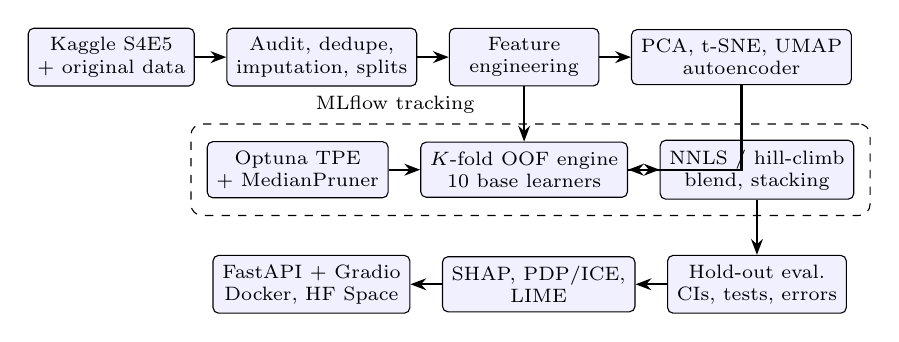
\begin{tikzpicture}[node distance=4mm and 4mm, every node/.style={font=\scriptsize},
  box/.style={draw, rounded corners=2pt, fill=blue!6, minimum width=19mm, minimum height=7mm, align=center},
  arr/.style={-{Stealth[length=2mm]}, thick}]
\node[box] (data) {Kaggle S4E5\\+ original data};
\node[box, right=of data] (prep) {Audit, dedupe,\\imputation, splits};
\node[box, right=of prep] (feat) {Feature\\engineering};
\node[box, right=of feat] (red) {PCA, t-SNE, UMAP\\autoencoder};
\node[box, below=7mm of feat] (cv) {$K$-fold OOF engine\\10 base learners};
\node[box, left=of cv] (opt) {Optuna TPE\\+ MedianPruner};
\node[box, right=of cv] (ens) {NNLS / hill-climb\\blend, stacking};
\node[box, below=7mm of ens] (eval) {Hold-out eval.\\CIs, tests, errors};
\node[box, left=of eval] (xai) {SHAP, PDP/ICE,\\LIME};
\node[box, left=of xai] (api) {FastAPI + Gradio\\Docker, HF Space};
\node[draw, dashed, rounded corners, fit=(opt)(cv)(ens), inner sep=2mm, label={[font=\scriptsize]above left:MLflow tracking}] {};
\draw[arr] (data)--(prep); \draw[arr] (prep)--(feat); \draw[arr] (feat)--(red);
\draw[arr] (feat)--(cv); \draw[arr] (red) |- (cv); \draw[arr] (opt)--(cv); \draw[arr] (cv)--(ens);
\draw[arr] (ens)--(eval); \draw[arr] (eval)--(xai); \draw[arr] (xai)--(api);
\end{tikzpicture}}
\caption{FloodGuard AI framework.}\label{fig:arch}
\end{figure}

\subsection{Data and preprocessing}
The Kaggle Playground Series S4E5 data~\cite{kaggles4e5} contain about 1.1 million rows with 20 integer factor scores and
the target \texttt{FloodProbability}; they were generated by a deep model trained on the original Flood Prediction Factors
dataset~\cite{floodorig}, which we merge as extra training rows (flag \texttt{is\_original}) and also use for external
validation. The audit checks the schema, data types and value ranges and removes exact duplicates
(Table~\ref{tab:audit}). Although S4E5 has no missing values, robustness is tested by injecting 5\% MCAR missingness
into a copy and comparing median, KNN and iterative imputation by downstream CV $R^2$; the best (\FGImputer) is part of
the serving pipeline. Outliers are flagged (IQR rule and Isolation Forest) but not removed. A 15\% hold-out set is
stratified by target deciles, and the remainder is split into \FGFolds{} stratified folds used for all out-of-fold work.

\subsection{Feature engineering}
For factors $x_{i1},\dots,x_{i20}$ we compute row statistics $s_i=\sum_j x_{ij}$, mean, standard deviation, min, max,
median, skewness, kurtosis and range, and counts $c_{ik}=\sum_j \mathbb{1}[x_{ij}\ge k]$ for $k=5,\dots,10$; the target is
strongly driven by $s_i$ (Spearman $\rho=\FGRhoSum$, Fig.~\ref{fig:corr}). Theme means (hydro-climatic, urban,
environmental, governance) and interactions such as Urbanization$\times$DrainageSystems add domain structure. Each factor
is also treated as a categorical: frequency encoding uses value counts of the training fold plus the unlabelled test set,
and the sorted factor vector gives a permutation-invariant view. Genuinely high-cardinality keys are formed from factor
pairs, $k_i=(x_{ia},x_{ib})$ (e.g.\ Urbanization$\times$DrainageSystems), whose levels far exceed those of a single factor
(Table~\ref{tab:audit}); each key is frequency- and target-encoded. Smoothed target encoding
\begin{equation}
\mathrm{TE}(v)=\frac{n_v\,\bar y_v+m\,\bar y}{n_v+m}
\end{equation}
is cross-fitted, so each training row is encoded with statistics from the other folds only. Mutual information and
permutation importance rank the \FGNumEngineered{} candidates; the top-$k$ ($k=\FGSelectedK$) is chosen by CV.

\subsection{Dimensionality reduction}
PCA quantifies the intrinsic dimensionality (scree and biplot, Fig.~\ref{fig:pca}); t-SNE~\cite{vandermaaten2008} and
UMAP~\cite{mcinnes2018} project the factors to 2-D, coloured by risk class. A symmetric autoencoder~\cite{hinton2006}
minimises $\frac{1}{n}\sum_i\lVert x_i-g(h(x_i))\rVert^2$; its 4-D bottleneck $h(x)$ feeds an Autoencoder$\to$LightGBM
model, and an ablation tests whether the embeddings help.

\subsection{Base learners}
Gradient boosting builds an additive model $\hat y_i^{(t)}=\hat y_i^{(t-1)}+\eta f_t(x_i)$. XGBoost minimises the
second-order approximation
\begin{equation}
\mathcal{L}^{(t)}\approx\sum_i\Big[g_i f_t(x_i)+\tfrac12 h_i f_t^2(x_i)\Big]+\gamma T+\tfrac12\lambda\lVert w\rVert^2,
\end{equation}
with gradient $g_i$ and Hessian $h_i$, giving optimal leaf weights $w_j^\ast=-G_j/(H_j+\lambda)$~\cite{chen2016}.
LightGBM adds leaf-wise growth with histogram binning~\cite{ke2017}, and CatBoost ordered boosting~\cite{prokhorenkova2018}.
Random forests average $B$ bootstrapped trees, $\hat f(x)=\frac1B\sum_b T_b(x;\Theta_b)$~\cite{breiman2001}, and Extra
Trees also randomise split thresholds~\cite{geurts2006}. Ridge/ElasticNet are linear baselines, and a PyTorch MLP
(BatchNorm, dropout, cosine learning-rate schedule, early stopping) is the deep-learning baseline.

\subsection{Ensemble layer}
Let $P\in\mathbb{R}^{n\times M}$ hold the out-of-fold (OOF) predictions of $M$ models. NNLS blending~\cite{breiman1996}
solves
\begin{equation}
\min_{w}\lVert Pw-y\rVert_2^2\quad\text{s.t. } w\ge 0,\ \mathbf{1}^\top w=1,
\end{equation}
hill climbing~\cite{caruana2004} greedily adds models with replacement, and stacking~\cite{wolpert1992} fits a Ridge or
LightGBM meta-learner $g$ on $z_i=(\hat f_1^{(-k(i))}(x_i),\dots,\hat f_M^{(-k(i))}(x_i),s_i,\sigma_i)$, scored by a
second CV level. A soft-voting classifier averages calibrated class probabilities of all members. The final strategy
(\FGEnsembleStrategy) is chosen by OOF $R^2$ and evaluated \emph{once} on the hold-out split.
Ground-truth risk classes are tertiles of the training target; prediction cut-offs are tuned on OOF predictions to
maximise macro-F1, and $P(\text{High}\mid\hat y)$ is calibrated by logistic regression on OOF predictions.

\subsection{Hyper-parameter search}
Optuna's multivariate TPE~\cite{bergstra2011,akiba2019} models $p(x\mid y)$ with densities $l(x)$ (good trials) and
$g(x)$ (others) and samples candidates maximising $l(x)/g(x)$; a median pruner stops trials whose fold scores fall below
the median. Studies are stored in SQLite (resumable) and every trial is an MLflow run. A GridSearchCV baseline on the
same rows and folds compares search strategies (Table~\ref{tab:search}).

\subsection{Explainability and evaluation}
Shapley values $\phi_j=\sum_{S\subseteq F\setminus\{j\}}\frac{|S|!(|F|-|S|-1)!}{|F|!}[v(S\cup\{j\})-v(S)]$ are computed
with TreeSHAP~\cite{lundberg2020} (global, interactions) and permutation sampling over the 20 raw factors for the deployed
ensemble~\cite{lundberg2017}. Metrics are $R^2$ (the competition metric), RMSE and MAE; macro-F1; and ROC-AUC, PR-AUC,
log-loss, Brier score and expected calibration error $\mathrm{ECE}=\sum_b\frac{n_b}{n}|\mathrm{acc}_b-\mathrm{conf}_b|$
for the High-risk flag~\cite{guo2017}. 95\% CIs use \FGBootstrap{} bootstrap resamples. The ensemble is compared with the
best single model by a paired bootstrap and a Wilcoxon signed-rank test over folds, and all models by a Friedman test with
the Nemenyi critical difference $\mathrm{CD}=q_\alpha\sqrt{k(k+1)/(6N)}$~\cite{demsar2006}.

% ----------------------------------------------------------- implementation
\section{Implementation and Experiments}
The framework is a Python package (\texttt{src/floodguard}) built on scikit-learn~\cite{pedregosa2011}, XGBoost, LightGBM,
CatBoost, PyTorch, Optuna, SHAP and MLflow, configured entirely by YAML (\texttt{configs/}). A single command runs the
stages \emph{download, prepare, features, reduce, tune, train, ensemble, evaluate, benchmark, explain, plots, report}.
Full experiments run on a Colab/Kaggle GPU runtime (hardware, library versions and stage runtimes in
Table~\ref{tab:env}); a synthetic smoke configuration verifies the whole pipeline on a CPU in minutes. The training split
has \FGTrainRows{} rows and the hold-out split \FGHoldoutRows{} rows.

\fgtable{environment}
Figs.~\ref{fig:shap}--\ref{fig:pdp} visualise model behaviour: SHAP shows how strongly the factor sum and its components
drive the prediction, and PDP/ICE curves show approximately monotone, near-linear factor effects.

\fgfig{03_correlation_dendrogram}{Spearman correlation of factors, factor sum and target with hierarchical clustering.}{fig:corr}
\fgfig{05_pca_scree_biplot}{PCA scree plot and biplot of the 20 factors.}{fig:pca}
\fgfig{06_tsne_umap}{t-SNE and UMAP projections coloured by risk class.}{fig:proj}
\fgfig{09_optuna}{Optuna optimisation history and hyper-parameter importance.}{fig:optuna}
\fgfigwide{14_shap_beeswarm_bar}{SHAP beeswarm and mean $|$SHAP$|$ importance (LightGBM, engineered features).}{fig:shap}
\fgfigwide{16_pdp_ice}{Partial dependence and ICE curves of the deployed ensemble for the most important factors.}{fig:pdp}

% ---------------------------------------------------------------- results
\section{Results and Comparative Analysis}
Table~\ref{tab:models} reports all models on the hold-out split. The selected \FGFinalModel{} attains
$R^2=\FGFinalRtwo$ [\FGFinalRtwoLo, \FGFinalRtwoHi], RMSE \FGFinalRMSE{} and MAE \FGFinalMAE{}; the linear model on the
factor sum alone reaches $R^2=\FGSumBaselineRtwo$, which quantifies how much of the signal the sum carries. The paired
bootstrap gives $\Delta R^2=\FGDeltaRtwo$ ($p=\FGPairedP$) over \FGBestSingle{}, and the Friedman test yields
$p=\FGFriedmanP$ (Table~\ref{tab:stats}, Fig.~\ref{fig:cd}). Table~\ref{tab:benchmark} places the result against simple
baselines, the Kaggle private leaderboard (top: \FGKaggleTop) and published studies. Trained on S4E5 only, the model
reaches $R^2=\FGExternalRtwo$ on the \FGExternalRows{} rows of the original dataset (Table~\ref{tab:external}).

\fgtable{model_comparison}
\fgtable{benchmark}
\fgtable{literature}
\fgtable{stat_tests}
\fgtable{ablation}
\fgtable{data_audit}
\fgtable{hyperparams}
\fgtable{search_comparison}
\fgtable{external}

For the risk classes the system reaches macro-F1 \FGMacroFone; the High-risk flag has ROC-AUC \FGRocAuc, PR-AUC
\FGPrAuc{} and ECE \FGECE{} (Figs.~\ref{fig:cm}--\ref{fig:cal}). Errors concentrate at the extremes of the target
(regression towards the mean) and near the class cut-offs (Fig.~\ref{fig:err}); the ablation (Table~\ref{tab:ablation})
measures the contribution of row features, target encoding, autoencoder embeddings and the original data.

\fgfig{11_confusion_matrix}{Confusion matrix of the risk classes (hold-out split).}{fig:cm}
\fgfig{12_roc_pr}{ROC and precision--recall curves of the High-risk flag.}{fig:roc}
\fgfig{13_calibration}{Reliability curve of $P(\text{High})$.}{fig:cal}
\fgfig{18_model_comparison}{Test $R^2$ with 95\% bootstrap confidence intervals.}{fig:comp}
\fgfig{21_critical_difference}{Average ranks and Nemenyi critical difference.}{fig:cd}
\fgfigwide{20_error_analysis}{Error analysis: residuals by target decile and MAE by theme quintile.}{fig:err}

% -------------------------------------------------------------- conclusion
\FloatBarrier  % keep every figure / table of the results inside the Results section
\section{Conclusion and Future Scope}
FloodGuard AI turns 20 flood-risk factors into a calibrated, explained risk estimate through a reproducible, tracked and
deployed ensemble pipeline. The experiments show (i) that engineered row statistics capture most of the signal, (ii) by
how much -- and how significantly -- blending and stacking improve on the best tuned single model, and (iii) where errors
remain. The service validates every input, returns a confidence interval from the spread of ensemble members, the top
SHAP drivers and mitigation actions, and runs in a Docker container on Hugging Face Spaces; in production it should be
monitored for data drift and recalibrated periodically.

\textbf{Limitations.} The S4E5 data are synthetically generated from the original dataset, and the factors are abstract
scores rather than physical measurements, so absolute results do not transfer to a specific city.
\textbf{Future work} includes real GIS/DEM, rainfall and drainage-network data for Indian cities, temporal forecasting
of flood events, and graph neural networks over drainage networks.

% -------------------------------------------------------------- references
\begin{thebibliography}{99}
\bibitem{mosavi2018} A. Mosavi, P. Ozturk, and K.-W. Chau, ``Flood prediction using machine learning models: Literature review,'' \emph{Water}, vol.~10, no.~11, Art.~no.~1536, 2018, doi: 10.3390/w10111536.
\bibitem{tehrany2014} M. S. Tehrany, B. Pradhan, and M. N. Jebur, ``Flood susceptibility mapping using a novel ensemble weights-of-evidence and support vector machine models in GIS,'' \emph{J. Hydrol.}, vol.~512, pp.~332--343, 2014, doi: 10.1016/j.jhydrol.2014.03.008.
\bibitem{khosravi2018} K. Khosravi \emph{et al.}, ``A comparative assessment of decision trees algorithms for flash flood susceptibility modeling at Haraz watershed, northern Iran,'' \emph{Sci. Total Environ.}, vol.~627, pp.~744--755, 2018, doi: 10.1016/j.scitotenv.2018.01.266.
\bibitem{ren2024} H. Ren \emph{et al.}, ``Flood susceptibility assessment with random sampling strategy in ensemble learning (RF and XGBoost),'' \emph{Remote Sens.}, vol.~16, no.~2, Art.~no.~320, 2024, doi: 10.3390/rs16020320.
\bibitem{rahimi2026} M. Rahimi \emph{et al.}, ``Integrating geospatial intelligence and machine learning for flood susceptibility mapping,'' \emph{Sci. Rep.}, vol.~16, Art.~no.~10228, 2026, doi: 10.1038/s41598-026-41014-3.
\bibitem{friedman2001} J. H. Friedman, ``Greedy function approximation: A gradient boosting machine,'' \emph{Ann. Statist.}, vol.~29, no.~5, pp.~1189--1232, 2001.
\bibitem{chen2016} T. Chen and C. Guestrin, ``XGBoost: A scalable tree boosting system,'' in \emph{Proc. 22nd ACM SIGKDD Int. Conf. Knowl. Discov. Data Min.}, 2016, pp.~785--794.
\bibitem{ke2017} G. Ke \emph{et al.}, ``LightGBM: A highly efficient gradient boosting decision tree,'' in \emph{Adv. Neural Inf. Process. Syst.}, vol.~30, 2017.
\bibitem{prokhorenkova2018} L. Prokhorenkova, G. Gusev, A. Vorobev, A. V. Dorogush, and A. Gulin, ``CatBoost: Unbiased boosting with categorical features,'' in \emph{Adv. Neural Inf. Process. Syst.}, vol.~31, 2018.
\bibitem{breiman2001} L. Breiman, ``Random forests,'' \emph{Mach. Learn.}, vol.~45, no.~1, pp.~5--32, 2001.
\bibitem{geurts2006} P. Geurts, D. Ernst, and L. Wehenkel, ``Extremely randomized trees,'' \emph{Mach. Learn.}, vol.~63, no.~1, pp.~3--42, 2006.
\bibitem{grinsztajn2022} L. Grinsztajn, E. Oyallon, and G. Varoquaux, ``Why do tree-based models still outperform deep learning on typical tabular data?'' in \emph{Adv. Neural Inf. Process. Syst. (Datasets and Benchmarks)}, vol.~35, 2022.
\bibitem{shwartz2022} R. Shwartz-Ziv and A. Armon, ``Tabular data: Deep learning is not all you need,'' \emph{Inf. Fusion}, vol.~81, pp.~84--90, 2022.
\bibitem{wolpert1992} D. H. Wolpert, ``Stacked generalization,'' \emph{Neural Netw.}, vol.~5, no.~2, pp.~241--259, 1992.
\bibitem{breiman1996} L. Breiman, ``Stacked regressions,'' \emph{Mach. Learn.}, vol.~24, no.~1, pp.~49--64, 1996.
\bibitem{caruana2004} R. Caruana, A. Niculescu-Mizil, G. Crew, and A. Ksikes, ``Ensemble selection from libraries of models,'' in \emph{Proc. 21st Int. Conf. Mach. Learn. (ICML)}, 2004.
\bibitem{bergstra2011} J. Bergstra, R. Bardenet, Y. Bengio, and B. K\'egl, ``Algorithms for hyper-parameter optimization,'' in \emph{Adv. Neural Inf. Process. Syst.}, vol.~24, 2011.
\bibitem{akiba2019} T. Akiba, S. Sano, T. Yanase, T. Ohta, and M. Koyama, ``Optuna: A next-generation hyperparameter optimization framework,'' in \emph{Proc. 25th ACM SIGKDD Int. Conf. Knowl. Discov. Data Min.}, 2019, pp.~2623--2631.
\bibitem{lundberg2017} S. M. Lundberg and S.-I. Lee, ``A unified approach to interpreting model predictions,'' in \emph{Adv. Neural Inf. Process. Syst.}, vol.~30, 2017.
\bibitem{lundberg2020} S. M. Lundberg \emph{et al.}, ``From local explanations to global understanding with explainable AI for trees,'' \emph{Nat. Mach. Intell.}, vol.~2, no.~1, pp.~56--67, 2020.
\bibitem{ribeiro2016} M. T. Ribeiro, S. Singh, and C. Guestrin, ```Why should I trust you?': Explaining the predictions of any classifier,'' in \emph{Proc. 22nd ACM SIGKDD Int. Conf. Knowl. Discov. Data Min.}, 2016, pp.~1135--1144.
\bibitem{vandermaaten2008} L. van der Maaten and G. Hinton, ``Visualizing data using t-SNE,'' \emph{J. Mach. Learn. Res.}, vol.~9, pp.~2579--2605, 2008.
\bibitem{mcinnes2018} L. McInnes, J. Healy, and J. Melville, ``UMAP: Uniform manifold approximation and projection for dimension reduction,'' arXiv:1802.03426, 2018.
\bibitem{hinton2006} G. E. Hinton and R. R. Salakhutdinov, ``Reducing the dimensionality of data with neural networks,'' \emph{Science}, vol.~313, no.~5786, pp.~504--507, 2006.
\bibitem{guo2017} C. Guo, G. Pleiss, Y. Sun, and K. Q. Weinberger, ``On calibration of modern neural networks,'' in \emph{Proc. 34th Int. Conf. Mach. Learn. (ICML)}, 2017, pp.~1321--1330.
\bibitem{demsar2006} J. Dem\v{s}ar, ``Statistical comparisons of classifiers over multiple data sets,'' \emph{J. Mach. Learn. Res.}, vol.~7, pp.~1--30, 2006.
\bibitem{pedregosa2011} F. Pedregosa \emph{et al.}, ``Scikit-learn: Machine learning in Python,'' \emph{J. Mach. Learn. Res.}, vol.~12, pp.~2825--2830, 2011.
\bibitem{kaggles4e5} W. Reade and A. Chow, ``Regression with a flood prediction dataset,'' Kaggle Playground Series, Season 4, Episode 5, 2024. [Online]. Available: \url{https://www.kaggle.com/competitions/playground-series-s4e5}
\bibitem{floodorig} naiyakhalid (Kaggle user), ``Flood prediction dataset,'' Kaggle. [Online]. Available: \url{https://www.kaggle.com/datasets/naiyakhalid/flood-prediction-dataset}
\end{thebibliography}

\end{document}
